% Autor: Alex Oster, Jonathan Sigrist, Luca Wiggering
% Datum: 2018-01
% basiert auf der Vorlage für Versuchsprotokolle von Simon May

%\includeonly{
%	tex/04_Titelseite,
%	tex/05_Gliederung,
%	tex/14_Kurzfassung,
%	tex/15_Theorie,
%	tex/16_Methoden,
%	tex/17_Ergebnisse,
%	tex/19_Zusammenfassung,
%	tex/20_Anhang,
%	tex/21_Literatur
%}

\documentclass[
	a4paper,                % Papierformat (DIN A4)
	titlepage=firstiscover, % Separate Titelseite
	captions=tableheading,  % \caption bei Tabellen immer als Überschrift setzen
	toc=bibliography,       % Literaturverzeichnis im Inhaltsverzeichnis aufführen
	toc=listof,             % Abbildungsverzeichnis etc. im Inhaltsverzeichnis aufführen
	oneside,                % Einseitig
	%twoside,               % Zweiseitig
	%twocolumn,             % Zweispaltig
	automark,               % Abschnittstitel automatisch in Kopfzeile einfügen
	12pt,                   % Schriftgröße (beliebige Größen mit „fontsize=Xpt“)
	english, ngerman,		% Sprache für z.B. Babel; ausgewählt: ngerman (letztgenannt)
	%draft=true             % Entwurf-Modus; markiert zu lange und zu kurze Zeilen
]{scrartcl}

% Autor: Simon May
% Datum: 2017-10-04

% --- Pakete einbinden
% --- Pakete erweitern LaTeX um zusätzliche Funktionen.
%     Dies ist ein Satz nützlicher Pakete.

% Silbentrennung etc.; Sprache wird durch Option bei \documentclass festgelegt
\usepackage{babel}
\usepackage{iftex}
\ifLuaTeX
	% Schriftart (Latin Modern)
	\usepackage{fontspec}
	\fontspec{Latin Modern Roman}
\else
	% Verwendung der Zeichentabelle T1 (für Sonderzeichen etc.)
	\usepackage[T1]{fontenc}
	% Legt die Eingabe-Zeichenkodierung fest, z.B. UTF-8
	\usepackage[utf8]{inputenc}
	% Schriftart (Latin Modern)
	\usepackage{lmodern}
	% Zusätzliche Sonderzeichen
	\usepackage{textcomp}
\fi

\usepackage{upgreek}
% Nutzen von +, -, *, / in \setlength u.ä. (z.B. \setlength{\a + 3cm})
\usepackage{calc}
% Wird benötigt, um \ifthenelse zu benutzen
\usepackage{xifthen}
% Optionen für eigene definierte Befehle
\usepackage{xparse}

% Verbessertes Aussehen des Schriftbilds durch kleine Anpassungen
\usepackage{microtype}
% Automatische Formatierung von Daten
\usepackage[useregional]{datetime2}
% Wird für Kopf- und Fußzeile benötigt
\usepackage{scrlayer-scrpage}
% Einfaches Wechseln zwischen unterschiedlichen Zeilenabständen
\usepackage{setspace}
% Optionen für Listen (enumerate, itemize, …)
\usepackage{enumitem}
% Automatische Anführungszeichen
\usepackage{csquotes}
% Zusätzliche Optionen für Tabellen (tabular)
\usepackage{array}

% Mathepaket (intlimits: Grenzen über/unter Integralzeichen)
\usepackage[intlimits]{amsmath}
% Mathe-Symbole, \mathbb etc.
\usepackage{amssymb}
% Weitere Mathebefehle
\usepackage{mathtools}
% „Schöne“ Brüche im Fließtext
\usepackage{xfrac}
% Ermöglicht die Nutzung von \SI{Zahl}{Einheit} u.a.
\usepackage{siunitx}
% Ermöglicht Nutzung von \pdv als Ableitungen
\usepackage{physics}
% Definition von Unicode-Symbolen; Nach [utf8]inputenc laden!
\usepackage{newunicodechar}
% Unicode-Formeln mit pdfLaTeX
% Autor: Simon May
% Datum: 2015-03-04

% Diese Datei ermöglicht es, Mathe-Symbole (z.B. \gamma) direkt als
% Sonderzeichen (d.h. γ) einzugeben

% silence unterdrückt Warnungen; vor hyperref laden
\usepackage{silence}
\WarningFilter[pdflatex-unicode-math]{newunicodechar}{Redefining Unicode character}
\ActivateWarningFilters[pdflatex-unicode-math]

\newunicodechar{†}{\dag}
\newunicodechar{‡}{\ddag}
\newunicodechar{…}{\ldots}
\newunicodechar{⋯}{\cdots}
\newunicodechar{⋮}{\vdots}
\newunicodechar{⋱}{\ddots}
\newunicodechar{⋰}{\iddots}
\newunicodechar{α}{\alpha}
\newunicodechar{β}{\beta}
\newunicodechar{γ}{\gamma}
\newunicodechar{δ}{\delta}
\newunicodechar{ε}{\varepsilon}
\newunicodechar{ϵ}{\epsilon}
\newunicodechar{ζ}{\zeta}
\newunicodechar{η}{\eta}
\newunicodechar{θ}{\theta}
\newunicodechar{ϑ}{\vartheta}
\newunicodechar{ι}{\iota}
\newunicodechar{κ}{\kappa}
\newunicodechar{ϰ}{\varkappa}
\newunicodechar{λ}{\lambda}
\newunicodechar{μ}{\mu}
\newunicodechar{ν}{\nu}
\newunicodechar{ξ}{\xi}
\newunicodechar{ο}{o}
\newunicodechar{π}{\pi}
\newunicodechar{ρ}{\rho}
\newunicodechar{ϱ}{\varrho}
\newunicodechar{σ}{\sigma}
\newunicodechar{τ}{\tau}
\newunicodechar{υ}{\upsilon}
\newunicodechar{φ}{\varphi}
\newunicodechar{ϕ}{\phi}
\newunicodechar{χ}{\chi}
\newunicodechar{ψ}{\psi}
\newunicodechar{ω}{\omega}
\newunicodechar{Α}{\mathrm{A}}
\newunicodechar{Β}{\mathrm{B}}
\newunicodechar{Γ}{\Gamma}
\newunicodechar{Δ}{\Delta}
\newunicodechar{Ε}{\mathrm{E}}
\newunicodechar{Ζ}{\mathrm{Z}}
\newunicodechar{Η}{\mathrm{H}}
\newunicodechar{Θ}{\Theta}
\newunicodechar{Ι}{\mathrm{I}}
\newunicodechar{Κ}{\mathrm{K}}
\newunicodechar{Λ}{\Lambda}
\newunicodechar{Μ}{\mathrm{M}}
\newunicodechar{Ν}{\mathrm{N}}
\newunicodechar{Ξ}{\Xi}
\newunicodechar{Ο}{\mathrm{O}}
\newunicodechar{Π}{\Pi}
\newunicodechar{Ρ}{\mathrm{P}}
\newunicodechar{Σ}{\Sigma}
\newunicodechar{Τ}{\mathrm{T}}
\newunicodechar{Υ}{\Upsilon}
\newunicodechar{Φ}{\Phi}
\newunicodechar{Χ}{\Chi}
\newunicodechar{Ψ}{\Psi}
\newunicodechar{Ω}{\Omega}
\newunicodechar{∑}{\sum}
\newunicodechar{∫}{\int}
\newunicodechar{∬}{\iint}
\newunicodechar{∭}{\iiint}
\newunicodechar{⨌}{\iiiint}
\newunicodechar{∮}{\oint}
\newunicodechar{∯}{\oiint}
\newunicodechar{∰}{\oiiint}
\newunicodechar{∇}{\nabla}
\newunicodechar{∂}{\partial}
\newunicodechar{√}{\sqrt}
\newunicodechar{∈}{\in}
\newunicodechar{∋}{\ni}
\newunicodechar{∉}{\notin}
\newunicodechar{∀}{\forall}
\newunicodechar{∃}{\exists}
\newunicodechar{∄}{\nexists}
\newunicodechar{∴}{\therefore}
\newunicodechar{∵}{\because}
\newunicodechar{〈}{\langle}
\newunicodechar{〉}{\rangle}
\newunicodechar{⌊}{\lfloor}
\newunicodechar{⌋}{\rfloor}
\newunicodechar{⌈}{\lceil}
\newunicodechar{⌉}{\rceil}
\newunicodechar{∼}{\sim}
\newunicodechar{∝}{\propto}
\newunicodechar{∞}{\infty}
\newunicodechar{ℵ}{\aleph}
\newunicodechar{ℏ}{\hbar}
\newunicodechar{℘}{\wp}
\newunicodechar{ℓ}{\ell}
\newunicodechar{∅}{\emptyset}
\newunicodechar{×}{\times}
\newunicodechar{⋅}{\cdot}
\newunicodechar{÷}{\div}
\newunicodechar{⋆}{\star}
\newunicodechar{∘}{\circ}
\newunicodechar{⋄}{\diamond}
\newunicodechar{⊕}{\oplus}
\newunicodechar{⊖}{\ominus}
\newunicodechar{⊗}{\otimes}
\newunicodechar{⊘}{\oslash}
\newunicodechar{⊙}{\odot}
\newunicodechar{±}{\pm}
\newunicodechar{∓}{\mp}
\newunicodechar{≈}{\approx}
\newunicodechar{≡}{\equiv}
\newunicodechar{≠}{\ne}
\newunicodechar{≥}{\ge}
\newunicodechar{≤}{\le}
\newunicodechar{≫}{\gg}
\newunicodechar{≪}{\ll}
\newunicodechar{⊂}{\subset}
\newunicodechar{⊃}{\supset}
\newunicodechar{⊆}{\subseteq}
\newunicodechar{⊇}{\supseteq}
\newunicodechar{⊈}{\nsubseteq}
\newunicodechar{⊉}{\nsupseteq}
\newunicodechar{≔}{\coloneqq}
\newunicodechar{≕}{\eqqcolon}
\newunicodechar{¬}{\neg}
\newunicodechar{∨}{\vee}
\newunicodechar{∧}{\wedge}
\newunicodechar{∪}{\cup}
\newunicodechar{∩}{\cap}
\newunicodechar{⋁}{\bigvee}
\newunicodechar{⋀}{\bigwedge}
\newunicodechar{⋃}{\bigcup}
\newunicodechar{⋂}{\bigcap}
\newunicodechar{⟂}{\perp}
\newunicodechar{∥}{\parallel}
\newunicodechar{∦}{\nparallel}
\newunicodechar{𝚤}{\imath}
\newunicodechar{𝚥}{\jmath}
\newunicodechar{⇔}{\Leftrightarrow}
\newunicodechar{⇕}{\Updownarrow}
\newunicodechar{⇐}{\Leftarrow}
\newunicodechar{⇒}{\Rightarrow}
\newunicodechar{⇑}{\Uparrow}
\newunicodechar{⇓}{\Downarrow}
\newunicodechar{↔}{\leftrightarrow}
\newunicodechar{↕}{\updownarrow}
\newunicodechar{←}{\leftarrow}
\newunicodechar{→}{\rightarrow}
\newunicodechar{↑}{\uparrow}
\newunicodechar{↓}{\downarrow}
\newunicodechar{⟷}{\longleftrightarrow}
\newunicodechar{⟵}{\longleftarrow}
\newunicodechar{⟶}{\longrightarrow}
\newunicodechar{⇇}{\leftleftarrows}
\newunicodechar{⇉}{\rightrightarrows}
\newunicodechar{⇈}{\upuparrows}
\newunicodechar{⇊}{\downdownarrows}
\newunicodechar{⟺}{\Longleftrightarrow}
\newunicodechar{⟸}{\Longleftarrow}
\newunicodechar{⟹}{\Longrightarrow}
\newunicodechar{↦}{\mapsto}
\newunicodechar{↤}{\mapsfrom}
\newunicodechar{⟼}{\longmapsto}
\newunicodechar{⟻}{\longmapsfrom}
\newunicodechar{⟾}{\Longmapsto}
\newunicodechar{⟽}{\Longmapsfrom}
\newunicodechar{↗}{\nearrow}
\newunicodechar{↖}{\nwarrow}
\newunicodechar{↘}{\searrow}
\newunicodechar{↙}{\swarrow}
\newunicodechar{↩}{\hookleftarrow}
\newunicodechar{↪}{\hookrightarrow}
\newunicodechar{↶}{\curvearrowleft}
\newunicodechar{↷}{\curvearrowright}
\newunicodechar{↺}{\circlearrowleft}
\newunicodechar{↻}{\circlearrowright}
\newunicodechar{↫}{\looparrowleft}
\newunicodechar{↬}{\looparrowright}
\newunicodechar{⇋}{\leftrightharpoons}
\newunicodechar{⇌}{\rightleftharpoons}
\newunicodechar{↼}{\leftharpoonup}
\newunicodechar{↽}{\leftharpoondown}
\newunicodechar{⇀}{\rightharpoonup}
\newunicodechar{⇁}{\rightharpoondown}
\newunicodechar{↿}{\upharpoonleft}
\newunicodechar{↾}{\upharpoonright}
\newunicodechar{⇃}{\downharpoonleft}
\newunicodechar{⇂}{\downharpoonright}
\newunicodechar{𝔸}{\mathbb{A}}
\newunicodechar{𝔹}{\mathbb{B}}
\newunicodechar{ℂ}{\mathbb{C}}
\newunicodechar{𝔻}{\mathbb{D}}
\newunicodechar{𝔼}{\mathbb{E}}
\newunicodechar{𝔽}{\mathbb{F}}
\newunicodechar{𝔾}{\mathbb{G}}
\newunicodechar{ℍ}{\mathbb{H}}
\newunicodechar{𝕀}{\mathbb{I}}
\newunicodechar{𝕁}{\mathbb{J}}
\newunicodechar{𝕂}{\mathbb{K}}
\newunicodechar{𝕃}{\mathbb{L}}
\newunicodechar{𝕄}{\mathbb{M}}
\newunicodechar{ℕ}{\mathbb{N}}
\newunicodechar{𝕆}{\mathbb{O}}
\newunicodechar{ℙ}{\mathbb{P}}
\newunicodechar{ℚ}{\mathbb{Q}}
\newunicodechar{ℝ}{\mathbb{R}}
\newunicodechar{𝕊}{\mathbb{S}}
\newunicodechar{𝕋}{\mathbb{T}}
\newunicodechar{𝕌}{\mathbb{U}}
\newunicodechar{𝕍}{\mathbb{V}}
\newunicodechar{𝕎}{\mathbb{W}}
\newunicodechar{𝕏}{\mathbb{X}}
\newunicodechar{𝕐}{\mathbb{Y}}
\newunicodechar{ℤ}{\mathbb{Z}}
\newunicodechar{𝒜}{\mathcal{A}}
\newunicodechar{ℬ}{\mathcal{B}}
\newunicodechar{𝒞}{\mathcal{C}}
\newunicodechar{𝒟}{\mathcal{D}}
\newunicodechar{ℰ}{\mathcal{E}}
\newunicodechar{ℱ}{\mathcal{F}}
\newunicodechar{𝒢}{\mathcal{G}}
\newunicodechar{ℋ}{\mathcal{H}}
\newunicodechar{ℐ}{\mathcal{I}}
\newunicodechar{𝒥}{\mathcal{J}}
\newunicodechar{𝒦}{\mathcal{K}}
\newunicodechar{ℒ}{\mathcal{L}}
\newunicodechar{ℳ}{\mathcal{M}}
\newunicodechar{𝒩}{\mathcal{N}}
\newunicodechar{𝒪}{\mathcal{O}}
\newunicodechar{𝒫}{\mathcal{P}}
\newunicodechar{𝒬}{\mathcal{Q}}
\newunicodechar{ℛ}{\mathcal{R}}
\newunicodechar{𝒮}{\mathcal{S}}
\newunicodechar{𝒯}{\mathcal{T}}
\newunicodechar{𝒰}{\mathcal{U}}
\newunicodechar{𝒱}{\mathcal{V}}
\newunicodechar{𝒲}{\mathcal{W}}
\newunicodechar{𝒳}{\mathcal{X}}
\newunicodechar{𝒴}{\mathcal{Y}}
\newunicodechar{𝒵}{\mathcal{Z}}
\newunicodechar{𝕬}{\mathfrak{A}}
\newunicodechar{𝕭}{\mathfrak{B}}
\newunicodechar{𝕮}{\mathfrak{C}}
\newunicodechar{𝕯}{\mathfrak{D}}
\newunicodechar{𝕰}{\mathfrak{E}}
\newunicodechar{𝕱}{\mathfrak{F}}
\newunicodechar{𝕲}{\mathfrak{G}}
\newunicodechar{𝕳}{\mathfrak{H}}
\newunicodechar{𝕴}{\mathfrak{I}}
\newunicodechar{𝕵}{\mathfrak{J}}
\newunicodechar{𝕶}{\mathfrak{K}}
\newunicodechar{𝕷}{\mathfrak{L}}
\newunicodechar{𝕸}{\mathfrak{M}}
\newunicodechar{𝕹}{\mathfrak{N}}
\newunicodechar{𝕺}{\mathfrak{O}}
\newunicodechar{𝕻}{\mathfrak{P}}
\newunicodechar{𝕼}{\mathfrak{Q}}
\newunicodechar{𝕽}{\mathfrak{R}}
\newunicodechar{𝕾}{\mathfrak{S}}
\newunicodechar{𝕿}{\mathfrak{T}}
\newunicodechar{𝖀}{\mathfrak{U}}
\newunicodechar{𝖁}{\mathfrak{V}}
\newunicodechar{𝖂}{\mathfrak{W}}
\newunicodechar{𝖃}{\mathfrak{X}}
\newunicodechar{𝖄}{\mathfrak{Y}}
\newunicodechar{𝖅}{\mathfrak{Z}}

\DeactivateWarningFilters[pdflatex-unicode-math]


% Farben
\usepackage{xcolor}
% Einbinden von Grafiken (\includegraphics)
\usepackage{graphicx}
% .tex-Dateien mit \includegraphics einbinden
\usepackage{gincltex}
% Größere Freiheiten bei Dateinamen mit \includegraphics
\usepackage{grffile}
% Abbildungen im Fließtext
\usepackage{wrapfig}
% Zitieren, Bibliographie (Biber als Bibliographie-Programm verwenden!)
\usepackage[backend=biber,sorting=none]{biblatex}
% Abbildungen nebeneinander (subfigure, subtable)
\usepackage{subcaption}
\usepackage{float}

% Verlinkt Textstellen im PDF-Dokument (sollte am Ende geladen werden)
\usepackage[unicode]{hyperref}
% „Schlaue“ Referenzen (nach hyperref laden!)
\usepackage{cleveref}
%PDF einbinden
%\usepackage{pdfpages}
%Graphiken zeichnen
%\usepackage{tikz}
%\usetikzlibrary{angles,quotes,babel,3d}
% --- Einstellungen
% -- LaTeX/KOMA
% 1,5-facher Zeilenabstand
\onehalfspacing
\recalctypearea
% Schrift bei Bildunterschriften ändern
\addtokomafont{caption}{\small}
\addtokomafont{captionlabel}{\bfseries}
% Nummerierung der Formeln entsprechend des Abschnitts (z.B. 1.1)
\numberwithin{equation}{section}
% „Verwaiste“ Zeilen am Seitenanfang/-Ende stärker vermeiden
\clubpenalty=1000
\widowpenalty=1000
% Auf mehrere Seiten aufgespaltene Fußnoten stärker vermeiden
\interfootnotelinepenalty=3000

% -- csquotes
% Anführungszeichen automatisch umwandeln
\MakeOuterQuote{"}

% -- siunitx
\sisetup{
	locale=DE,
	separate-uncertainty,
	output-product=\cdot,
	quotient-mode=fraction,
	per-mode=fraction,
	fraction-function=\sfrac
}

% -- hyperref
\hypersetup{
	% Links/Verweise mit Kasten der Dicke 0.5pt versehen
	pdfborder={0 0 0.5}
}

% -- cleveref
\crefname{equation}{}{}
\Crefname{equation}{}{}

% -- biblatex (Literaturverzeichnis)
\IfFileExists{res/literatur.bib}{
	\addbibresource{res/literatur.bib}
}{}

\AtEndPreamble{
	% Kopf- und Fußzeile konfigurieren
	\ifthenelse{\boolean{showHeader}}{
		\KOMAoptions{headsepline}
		\recalctypearea
		\automark{section}
		% Innenseite der Kopfzeile
		\ihead{\headmark}
		% Mitte der Kopfzeile
		\chead{}
		% Außenseite der Kopfzeile
		\ohead{\usekomafont{pagehead}\varAutor}
	}{}
	% Innnenseite der Fußzeile
	\ifoot{}
	% Mitte der Fußzeile          
	\cfoot{-~\pagemark~-}
	% Außenseite der Fußzeile
	\ofoot{}

	% Metadaten für die PDF-Datei
	\hypersetup{
		pdftitle={Versuchsprotokoll: \varName},
		pdfauthor={\varAutor},
		pdfsubject={Masterpraktikum},
		pdfkeywords={Physik, Münster, Praktikum, Versuchsprotokoll}
	}
}


% Autor: Simon May
% Datum: 2017-10-05

% Eigene Befehle eignen sich gut, um Abkürzungen für lange Befehle zu erstellen.
% So vermeidet man, dass man immer wieder dasselbe Konstrukt kopieren und
% einfügen muss und, wenn man dann doch etwas ändern will, an zahllosen Stellen
% im Dokument dieselbe Änderung vornehmen muss.
% Die Syntax ist die folgende:
% \newcommand{neuer Befahl}[Anzahl Parameter (optional)]{Inhalt}
% Das folgende Beispiel fügt ein Bild mit bestimmten vorgegebenen Optionen ein:
\newcommand{\centeredImage}[1]{
	\begin{figure}
		\centering
		\includegraphics[width=0.5\textwidth]{#1}
	\end{figure}
}
% #1 ist dabei ein Parameter, den man \centeredImage übergeben muss, also:
% \centeredImage{...}
% Benötigt man keine Parameter, dann lässt man [1] weg. Werden zusätzliche
% Parameter benötigt, dann kann man die Zahl auf maximal 9 erhöhen.

% Ein Befehl, um eine E-Mail-Adresse darzustellen bzw. automatisch zu verlinken
\newcommand{\email}[1]{\href{mailto:#1}{\texttt{#1}}}

% \arsinh etc.
\newcommand*{\arsinh}{\operatorname{arsinh}}
\newcommand*{\arcosh}{\operatorname{arcosh}}
\newcommand*{\artanh}{\operatorname{artanh}}
\newcommand*{\const}{\text{const.}}

% Autor: Simon May
% Datum: 2016-10-13
% Der Befehl \newcommand kann auch benutzt werden, um „Variablen“ zu definieren:

% Nummer laut Praktikumsheft:
%\newcommand*{\varNum}{V07}
% Name laut Praktikumsheft:
\newcommand*{\varName}{Elektronenmikroskopie} %"\\" in hyperref gives warnings and is removed.
% Datum der Durchführung (Format: JJJJ-MM-TT):
\newcommand*{\varDatum}{10.09.2020}
% Autoren des Protokolls:
\newcommand*{\varAutor}{N. Wydra, A. Oster, L. Segger}
\newcommand*{\varNameA}{Norbert Wydra}
\newcommand*{\varNameB}{Alex Oster}
\newcommand*{\varNameC}{Leonhard Segger}
% Nummer der eigenen Gruppe:
\newcommand*{\varGruppe}{Blockpraktikum Biophysik, Gruppe F}
% E-Mail-Adressen der Autoren (kommagetrennt ohne Leerzeichen!):
\newcommand{\varEmail}{l.segger@uni--muenster.de,a\_oste16@uni--muenster.de, n\_wydr01@uni--muenster.de}
\newcommand{\varEmailA}{n\_wydr01@uni--muenster.de}
\newcommand{\varEmailB}{a\_oste16@uni--muenster.de}
\newcommand{\varEmailC}{l.segger@uni--muenster.de}
%betreuer Name
\newcommand{\varBetreuer}{\normalsize betreut von Dr. Yaroslav Tsytsyura}
% E-Mail-Adresse anzeigen (true/false):
\newcommand*{\varZeigeEmail}{true}
% Kopfzeile anzeigen (true/false):
\newcommand*{\varZeigeKopfzeile}{true}
% Inhaltsverzeichnis anzeigen (true/false):
\newcommand*{\varZeigeInhaltsverzeichnis}{true}
% Literaturverzeichnis anzeigen (true/false):
\newcommand*{\varZeigeLiteraturverzeichnis}{true}

\usepackage{upgreek}

\newboolean{showEmail}
\setboolean{showEmail}{\varZeigeEmail}
\newboolean{showHeader}
\setboolean{showHeader}{\varZeigeKopfzeile}
\newboolean{showTOC}
\setboolean{showTOC}{\varZeigeInhaltsverzeichnis}
\newboolean{showBibliography}
\setboolean{showBibliography}{\varZeigeLiteraturverzeichnis}

\renewcommand\maketitle{}

\bibliography{lit/literatur}
\setlength\parindent{0pt}

\begin{document}

	% Römische Seitenzahlen für Titelseite/Inhaltsverzeichnis
	\pagenumbering{roman}
	% Zunächst ohne Kopf-/Fußzeile
	\pagestyle{scrplain}

	% --- Titelseite einbinden
	%     Falls die Datei „res/titelbild.pdf“ existiert, wird sie auf der Titelseite
	%     eingefügt
	\IfFileExists{tex/04_Titelseite.tex}{
		% Autor: Simon May
% Datum: 2017-10-05

% Befehl, um die E-Mail-Adressen auf der Titelseite darzustellen
\makeatletter
\newcommand*{\protokollemailparse}[1]{%
	\@for\@tempa:=#1\do{%
		\normalsize\email{\@tempa}\\
	}%
}
\makeatother

\begin{titlepage}
	\centering
	{\scshape\LARGE Versuchsbericht zu \par}
	\vspace{1cm}
	{\scshape\huge \varName\par}
	\vspace{2.5cm}
	{\LARGE \varGruppe\par}
	\vspace{0.5cm}
	{\large \varNameA {} (\varEmailA) \par}
	{\large \varNameB {} (\varEmailB) \par}
	{\large \varNameC {} (\varEmailC) \par}
	\vfill
	durchgeführt am \varDatum\par
	{\large \varBetreuer}
	\vfill
	{\large \today\par}
\end{titlepage}

% Falls die Datei „res/titelbild.pdf“ existiert, wird sie hier eingefügt
\IfFileExists{res/titelbild.pdf}{
	\publishers{\vspace{2ex}\includegraphics[width=0.75\textwidth]{res/titelbild.pdf}}
}{}

\maketitle

	}{}
	
% --- Inhaltsverzeichnis einbinden
\ifthenelse{\boolean{showTOC}}{
		\tableofcontents
		\clearpage
	}{}


	% Zurücksetzen der Seitenzahlen auf arabische Ziffern
	\pagenumbering{arabic}
	% Ab hier mit Kopf- und Fußzeile
	\pagestyle{scrheadings}

	\section{Einleitung}
	% Hypothese	und deren Ergebnis, wenn Hypothese ist, dass nur Theorie erfüllt, sagen: Erwartung: Theorie aus einführung (mit reflink) erfüllt
	% Ergebnisse, auch Zahlen, mindestens wenn's halbwegs Sinn ergibt
	% Was wurde gemacht
	% manche leute wollen Passiv oder "man", manche nicht


  MALDI (Matrix-unterstützte Laser-Desorption/Ionisation) erlaubt es, Moleküle in die Gasphase zu überführen und zu ionisieren.
  In der MALDI wird dies erreicht, indem Analytmoleküle zusammen mit einer Matrix in einen Kristall eingebaut werden, welcher dann mit einem Laser beschossen wird.
  In der Gasphase können sie dann mittels eines Massenspektrometers (hier eines Flugzeitspektrometer) nach ihrem Masse-zu-Ladung-Verhältnis $m/z$ aufgetrennt und nachgewiesen werden.

  Dieses Verfahren lässt verschiedene Parameter offen, die für Ionenausbeute, geringe Ionenfragmentierung, Signal-Rausch-Verhältnis, Massenauflösung und Massengenauigkeit optimiert werden können.
  Dementsprechend sollen hier die Parameter Analytverdünnung, Art der verwendeten Matrix und Modus des Flugzeitspektrometers verändert werden, um die Abhängigkeit jener Größen zu untersuchen.

  Des Weiteren ist es möglich, räumlich aufgelöste MALDI-Messungen durchzuführen, indem eine dünn geschnittene Probe komplett mit Matrix beschichtet wird und dann rasterförmig MALDI-Spektren für jeden Pixel des Rasters aufgenommen werden.
  Dies kann beispielsweise erlauben, während Operationen festzustellen, welche Bereiche eines Organs von Krebs befallen sind und welche nicht.
  Hierfür muss bekannt sein, wie sich die Häufigkeiten bestimmter Ionen in Tumorzellen von denen in gesunden Zellen unterscheiden.
  Solange dies bekannt ist, ist es jedoch nicht nötig, sich auf Anfärbungen und Erfahrung des/der OP-Leiter:in zu verlassen.

  In diesem Versuch soll ein Coronal-Schnitt eines Mäusehirns verwendet werden, um Strukturen innerhalb der Probe zu identifizieren und den Schnitt innerhalb des Hirns zu lokalisieren.
  Dazu werden Referenzbilder, welche anhand von verschiedenen Färbungen entwickelt wurden, verwendet.

  Aufgrund von Matrixeffekten und probenabhängiger schwankender Ionenausbeiten ist es jedoch schwierig, mit der MALDI eine Quantifizierung der Konzentration der gemessenen Ionen in der Probe vorzunehmen.

	\input{tex/13_Durchführung}
	\clearpage
\section{Auswertung}

\subsection{Lipide}

Untersucht wurden im Folgenden die Peaks von [PC(32:0)+H]$^+$ bei \SI{734.562}{} und [PC(34:1)+H]$^+$ bei \SI{760,578}{}.
In \cref{fig_broken} sind zwei Massenspektren dargestellt, die sich insofern von den meisten aufgenommenen Spektren unterscheiden, als dass ein starkes Untergrundsignal vorliegt, welches entweder auf Verunreinigungen in der Probe zurückzuführen ist.
Auch denkbar ist, dass bei sehr geringer Analytkonzentration mehr Untergrund ionisiert und gemessen wird.
In \cref{fig_very_broken} sind dabei die zu untersuchenden Peaks nicht mehr zu erkennen, weshalb dieses und ein weiteres Spektrum dieser Art nicht verwendet werden können.
Im Gegensatz dazu ist in \cref{fig_fine_broken} das Signal noch deutlich zu erkennen, weshalb die sechs Spektren dieser Art ausgewertet werden.

\begin{figure}[!ht]
    \centering
    \begin{subfigure}{0.495\textwidth}
        \centering
        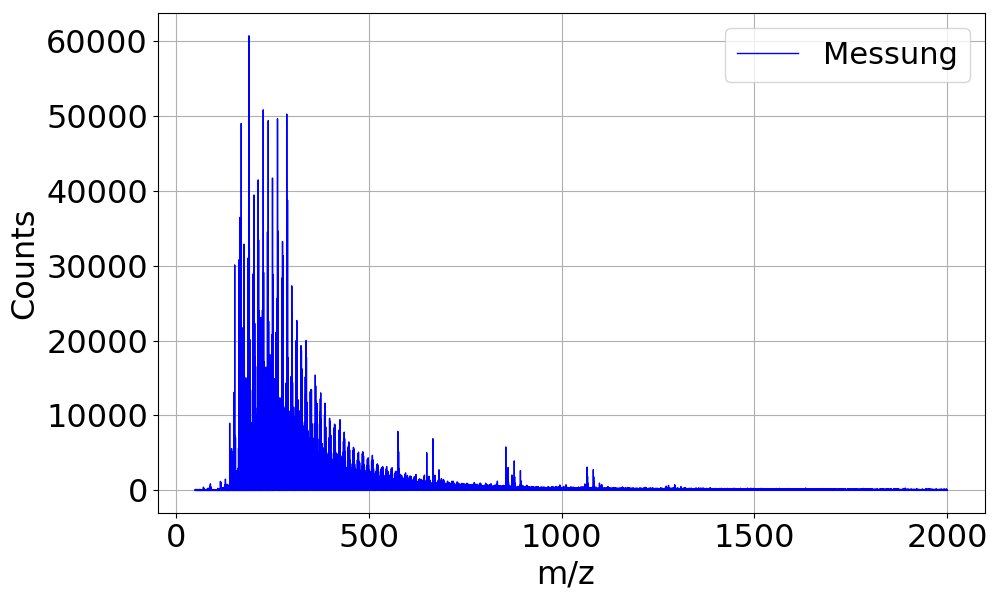
\includegraphics[width=1.0\textwidth]{img/b11_S_broken}
        \caption{CHCA $10^{-6}$ \si{\mole \per \liter}}
        \label{fig_very_broken}
    \end{subfigure}
    \begin{subfigure}{0.495\textwidth}
        \centering
        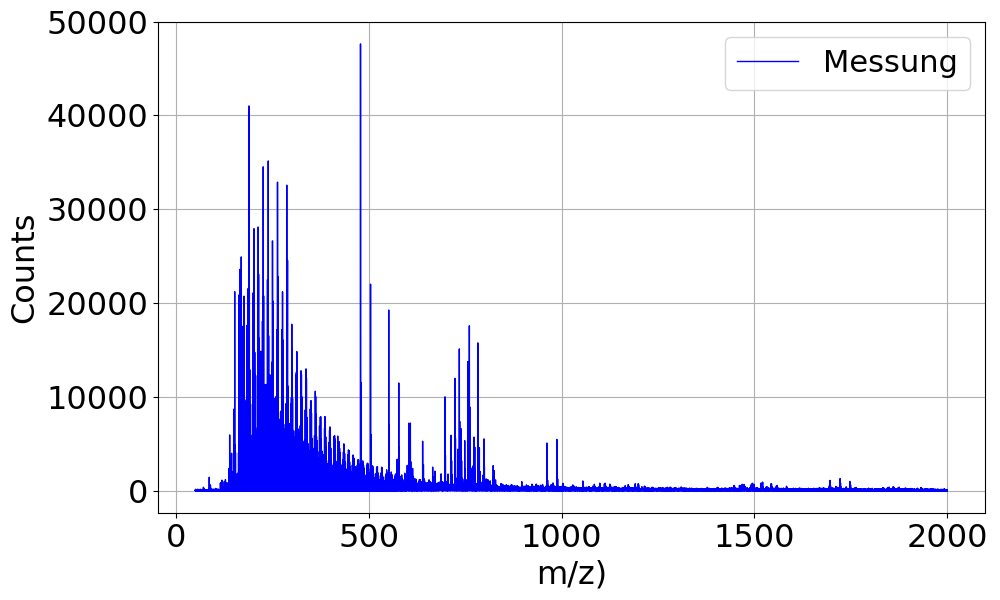
\includegraphics[width=1.0\textwidth]{img/C11_S_broken_but_fine}
        \caption{CHCA $10^{-5}$ \si{\mole \per \liter}}
        \label{fig_fine_broken}
    \end{subfigure}
    \caption{Zwei Massenspektren mit großem Untergrundsignal bei Matrix CHCA und unterschiedlichen Analytkonzentrationen. Beide im S-Modus.}
    \label{fig_broken}
\end{figure}

Zur Auswertung der Spektren wird für jedes Spektrum und beide untersuchte Peaks ein lokaler Gauß-Fit durchgeführt, von denen einer in \cref{fig_gaussfit} abgebildet ist.
Aus den Fit-Parametern werden Signalstärke, Peakposition (Masse-zu-Ladung-Verhältnis), Halbwertsbreite und ein als lokal konstant angenommener Untergrund entnommen.

\begin{figure}[!ht]
    \centering
    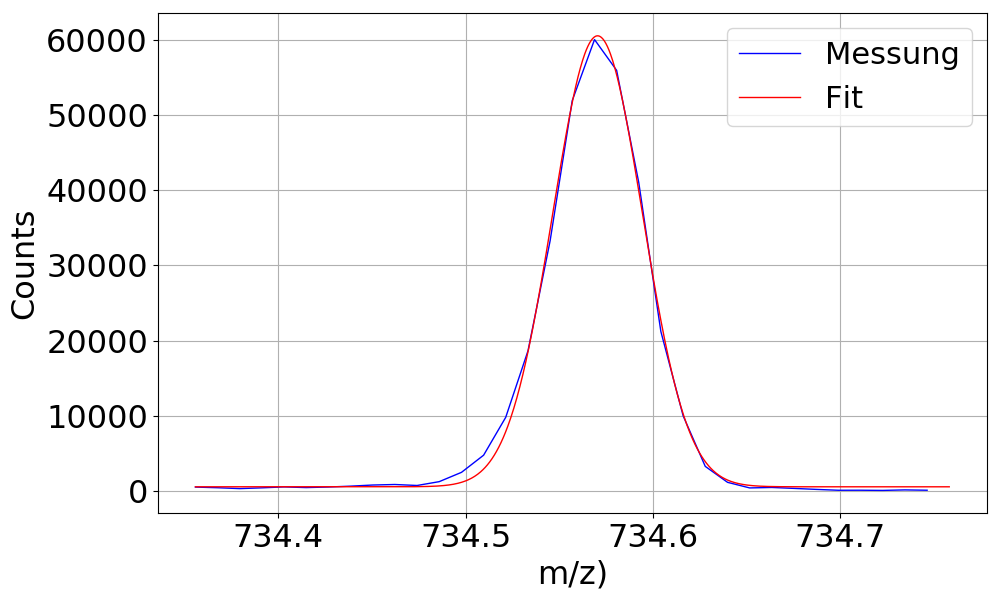
\includegraphics[width=0.6\textwidth]{img/a04_S_gaussfit}
    \caption{Gauß-Fit bei Matrix DHB und einer Analytkonzentration von $10^{-7}$ \si{\mole \per \liter}.}
    \label{fig_gaussfit}
\end{figure}

Sofern mindestens zwei Spektren zur Verfügung stehen, wird für die Ergebnisse ein Mittelwert und die Standardunsicherheit bestimmt und im Folgenden als Unsicherheit verwendet.
Eine Tabelle mit den Ergebnissen aller Fits bei allen Spektren findet sich in \cref{sec:anhang}.

Um die Massenauflösung $R=\frac{m}{\Delta m}$ zu bestimmen und den HR-Modus mit dem S-Modus zu vergleichen, wird jeweils das Masse-zu-Ladung-Verhältnis durch die Halbwertsbreite geteilt.
Die Ergebnisse sind in \cref{tab:HR-S-vgl} dargestellt.
Es ist deutlich zu erkennen, dass die Massenauflösung im HR-Modus wie erwartet deutlich größer ist.
Außerdem ist sie bei Verwendung von  DHB als Matrix im S-Modus etwas größer als bei CHCA und im HR-Modus etwas kleiner.
Es ist auch sichtbar, dass die Standardunsicherheit im S-Modus um etwa eine Größenordnung geringer ist, also die Massengenauigkeit höher ist.

\begin{table}[H]
	\centering
	\caption{Ergebnisse aus den Fits ausgewählter Peaks in den Massenspektren nach Matrix und Modus des Flugzeitspektrometers. Die Verdünnungsstufe beträgt $10^{-4}$ \si{\mole \per \liter}.}
	   \begin{tabular}{c | c | c | c }
      Modus & Matrix & $m/z$ & Massenauflösung $R$ \\ \hline
      S & CHCA & \SI{734,56818 \pm 0,00018}{} & \SI{12717 \pm 57}{} \\
        &      & \SI{760,58348 \pm 0,00020}{} & \SI{12788 \pm 306}{} \\
        & DHB  & \SI{734,56951 \pm 0,00011}{} & \SI{14645 \pm 450}{} \\
        &      & \SI{760,58491 \pm 0,00022}{} & \SI{14634 \pm 540}{} \\
      HR& CHCA & \SI{734,5653  \pm 0,0014}{}  & \SI{39841 \pm 657}{} \\
        &      & \SI{760,5811  \pm 0,0010}{}  & \SI{38488 \pm 2688}{} \\
        & DHB  & \SI{734,5643  \pm 0,0018}{}  & \SI{36596 \pm 2531}{} \\
        &      & \SI{760,5801  \pm 0,0011}{}  & \SI{36686 \pm 1287}{} \\
	\end{tabular}
	\label{tab:HR-S-vgl}
\end{table}

Nun soll noch Massengenauigkeit und Massenrichtigkeit bei verschiedenen Verdünnungsstufen verglichen werden.
Hierfür wird der Sensitivity-Modus verwendet, weil hier ein besseres Signal-Rausch-Verhältnis zu erwarten ist und die Massenauflösung auch hier groß genug ist, um die betrachteten Peaks eindeutig voneinander trennen zu können.
Die Massengenauigkeit wird wie oben über die Standardunsicherheit bestimmt.
Wenn nur ein Spektrum zur Verfügung steht, wird die Unsicherheit, die sich aus dem Fit ergibt, verwendet.
In diesem Fall werden die Daten mit einem $*$ gekennzeichnet.
Für die Massenrichtigkeit wird die Differenz zwischen Mittelwert der gemessenen Masse-zu-Ladung-Verhältnisse und dem erwarteten exakten Masse-zu-Ladung-Verhältnis des jeweiligen Moleküls gebildet.
Da für die exakte Masse des Moleküls Werte mit drei Nachkommastellen angegeben wurden, ergibt sich für die Massenrichtigkeit eine zusätzliche digitale Unsicherheit von $\approxeq \SI{0.0003}{}$.
Außerdem wird das Signal-Rausch-Verhältnis bestimmt, indem die Höhe des gefitteten Gauß-Peaks durch die Größe des lokalen konstanten Untergrunds geteilt wird.
Wie in \cref{fig_gaussfit} zu erkennen ist, ist die Annahme eines konstanten Untergrund in guter Näherung gerechtfertigt und da die betrachteten Peaks deutlich voneinander getrennt sind, ist auch nicht zu befürchten, dass ein Teil der Höhe der Peaks auf eine Überlappung mit anderen Peaks zurückzuführen ist.
In einigen Fällen treten jedoch deutlich kleinere Peaks im Bereich des lokalen Fits auf, die mittels dieser Methode nur als Anteil am konstanten Untergrund gewertet werden.
Auch hier wird, wenn möglich, ein Mittelwert verwendet und die Standardunsicherheit angegeben.
Die Ergebnisse sind in \cref{tab:verduennungen} aufgeführt.

\begin{table}[H]
	\centering
	\caption{Massengenauigkeit, -richtigkeit und Signal-Rausch-Verhältnis (SRV) aus den Fits ausgewählter Peaks in den Massenspektren nach Matrix und Verdünnungsstufe. Die Spektren wurden im Sensitivity-Modus aufgenommen. $*$ markiert, wenn für die Berechnung nur ein Spektrum zur Verfügung steht, weshalb hier der Fehler aus dem Fit verwendet wird. Verdünnung in \si{\mole \per \liter}}
	   \begin{tabular}{c | c | c | c  | c | c}
      Verd. & Matrix & $m/z$ & Massenrichtigkeit & SRV \\ \hline
      $10^{-4}$ & CHCA & \SI{734,56818 \pm 0,00018}{} & \SI{0,00619 \pm 0,00034}{} & \SI{110,3 \pm 3,4}{}\\
                &      & \SI{760,58348 \pm 0,00020}{} & \SI{0,00548 \pm 0,00035}{} & \SI{133 \pm 18}{}\\
                & DHB  & \SI{734,56951 \pm 0,00011}{} & \SI{0,00751 \pm 0,00031}{} & \SI{136,8 \pm 9,5}{}\\
                &      & \SI{760,58491 \pm 0,00022}{} & \SI{0,00691 \pm 0,00037}{} & \SI{142,6 \pm 3,5}{}\\
      $10^{-5}$ & CHCA & \SI{734,57021 \pm 0,00023}{} $*$ & \SI{0,00821 \pm 0,00037}{} & \SI{65 \pm 11}{}\\
                &      & \SI{760,58573 \pm 0,00025}{} $*$ & \SI{0,00773 \pm 0,00038}{} & \SI{74 \pm 12}{} \\
                &  DHB & \SI{734,57025 \pm 0,00024}{} $*$ & \SI{0,00825 \pm 0,00038}{} & \SI{81 \pm 16}{}\\
                &      & \SI{760,58590 \pm 0,00022}{} $*$ & \SI{0,00790 \pm 0,00036}{} & \SI{108 \pm 33}{}\\
      $10^{-6}$ & DHB  & \SI{734,56906 \pm 0,0007 }{} $*$ & \SI{0,00706 \pm 0,00076}{} & \SI{17 \pm 2}{}\\
                &      & \SI{760,58529 \pm 0,0006 }{} $*$ & \SI{0,00729 \pm 0,00067}{} & \SI{21 \pm 3}{}\\
      $10^{-7}$ & DHB  & \SI{734,57022 \pm 0,00030}{} & \SI{0,00822 \pm 0,00042}{} & \SI{93 \pm 11}{}\\
                &      & \SI{760,58569 \pm 0,00027}{} & \SI{0,00769 \pm 0,00039}{} & \SI{71 \pm 27}{}\\
	\end{tabular}
	\label{tab:verduennungen}
\end{table}

Für den Vergleich der Verdünnungsstufen soll sich auf DHB konzentriert werden, da hier mehr Spektren aufgenommen wurden.
Die Massengenauigkeit scheint mit sinkender Verdünnung schlechter zu werden (der Zahlenwert der Standardunsicherheit nimmt zu).
Dies kann jedoch aufgrund mangelnder Spektren nur an zwei Verdünnungsstufen festgemacht werden.

Bei der Massenrichtigkeit ist kein signifikanter Trend zu erkennen.
Dies ist nicht verwunderlich, da die Massenrichtigkeit vor allem von der Kalibrierung abhängt, welche für alle aufgenommenen Spektren gleich ist.

Anhand der Daten für die Verdünnungsstufen $10^{-4}$, $10^{-5}$ und $10^{-6}$ \si{\mole \per \liter} lässt sich feststellen, dass das Signal-Rausch-Verhältnis mit der Analytkonzentration deutlich abnimmt.
Bei DHB wurde bei der Verdünnungsstufe von $10^{-7}$ \si{\mole \per \liter} vermutlich ein Fehler in der Präparation gemacht, da hier der Trend gebrochen wird und das Signal-Rausch-Verhältnis wieder deutlich ansteigt
\par

Anhand der vorherigen Ergebnisse wird als Spektrum mit optimalen Bedingungen für ein Übersichtsbild DHB bei einer Verdünnungsstufe von $10^{-4}$ \si{\mole \per \liter} im Sensitivity-Modus gewählt.
In \cref{fig_gesamtspekt} ist dieses Spektrum dargestellt und der rote Ausschnitt ist in \cref{fig:teilspekt} vergrößert dargestellt.
Dort wurden die Peaks den verschiedenen Lipidspezies zugeordnet.

\begin{figure}[!ht]
    \centering
    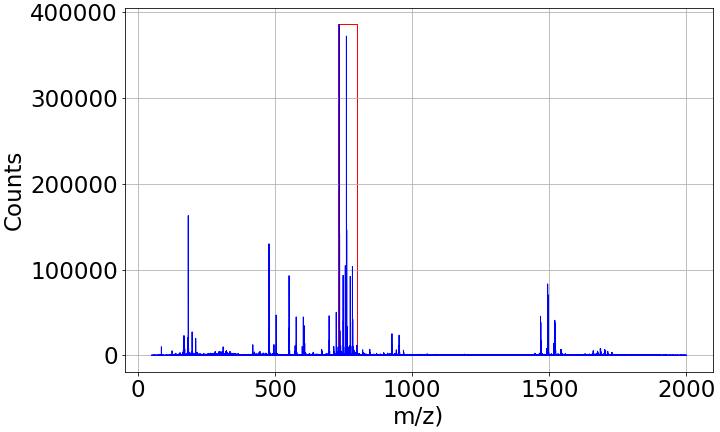
\includegraphics[width=1\textwidth]{img/overview-D02_Oben_S}
    \caption{Gemessenes Gesamtspektrum bei Matrix DHB, Verdünnungsstufe $10^{-4}$ \si{\mole \per \liter} und im Sensitivity-Modus.}
    \label{fig_gesamtspekt}
\end{figure}

\begin{figure}[!ht]
    \centering
    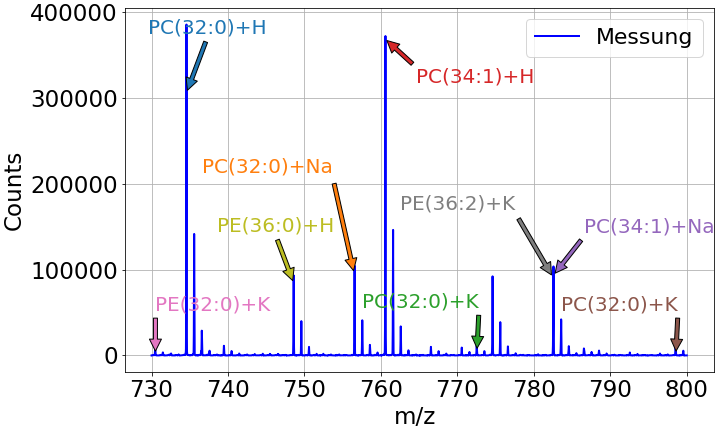
\includegraphics[width=1\textwidth]{img/overview_zoom-D02_Oben_S}
    \caption{Annotierter Ausschnitt aus dem gemessenen Spektrum bei Matrix DHB, Verdünnungsstufe $10^{-4}$ \si{\mole \per \liter} und im Sensitivity-Modus.}
    \label{fig:teilspekt}
\end{figure}


\subsection{Imaging}

Es ist möglich, das Bild über die gemessene Gesamtionenzahl (TIC, Total Ion Count) des im jeweiligen Pixel zu normieren. %ich denke, dass Gesamtzahl aller Ionen im Pixel und nicht des einzelnen Ions im Bild gemeint ist.
Dies verursacht hier nur eine geringfügige Änderung des Bildes, erlaubt aber zu erkennen, falls der Probenschnitt nicht gerade geschnitten ist, da in diesem Fall manche Pixel weniger Ionenausbeute hätten.

In \cref{fig:hirn1} ist das Imaging-Bild bei Auswahl von Ionen mit Masse-zu-Ladung-Verhältnis von \SI{772.546}{} dargestellt.
Anhand der Referenzbilder von \emph{reference atlas viewers} \cite{mouse-brain-map} lässt sich dies etwa Coronal-Ebene 118 (Bregma \SI{-6,455}{mm}) zuordnen.
Das Referenzbild ist in \cref{fig:hirn-ref} abgebildet.
Dabei fällt auf, dass im oberen Bereich des Bildes die Probe leicht beschädigt ist.

\begin{figure}[!ht]
    \centering
    \begin{subfigure}{0.65\textwidth}
        \centering
        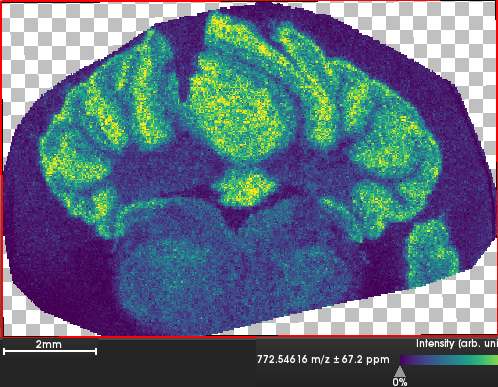
\includegraphics[width=1\textwidth]{raw/hirn/Hirn772_crop}
        \caption{MALDI-Aufnahme}
        \label{fig:hirn1}
    \end{subfigure}
    \begin{subfigure}{0.65\textwidth}
        \centering
        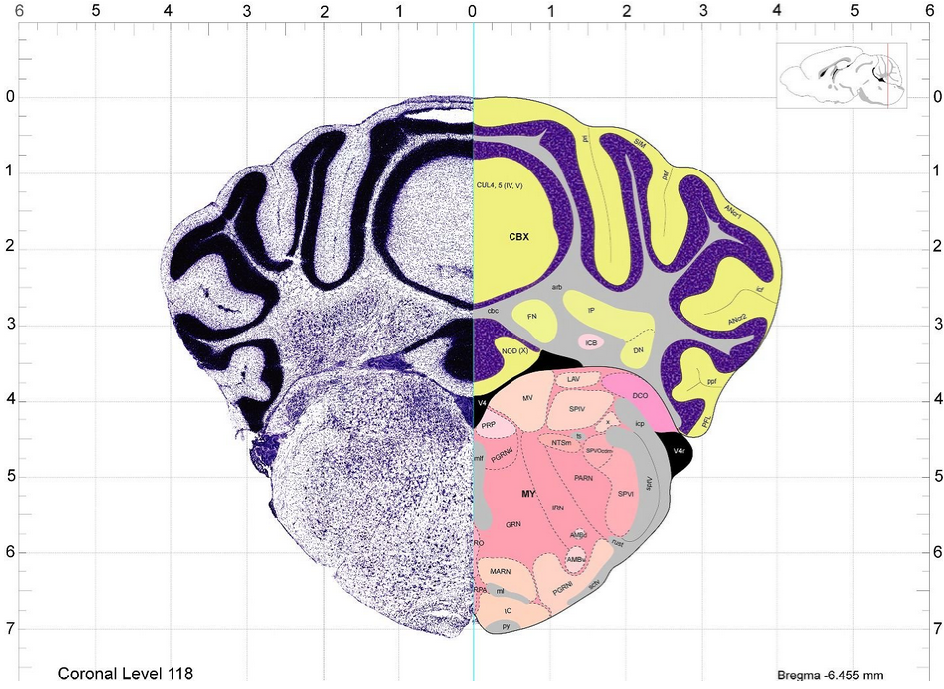
\includegraphics[width=1\textwidth]{img/coronal_ref}
        \caption{Referenzbild}
        \label{fig:hirn-ref}
    \end{subfigure}
    \caption{(a) MALDI-Imaging-Aufnahme eines Coronal-Schnittes eines Mäusehirns. (b) Zugeordnetes Referenzbild des verwendeten Coronal-Schnittes. \cite{mouse-brain-map}}
    \label{fig:hirn-vgl}
\end{figure}

Nun werden mithilfe des \emph{interactive atlas viewers} die bei der jeweiligen Ionenauswahl sichtbaren Bereiche identifiziert und in \cref{fig:hirn-ann} beschriftet dargestellt.
Dabei wurden die Ionen mit $m/z$ von \SI{838.60667}{} und \SI{872.52693} ausgewählt und in unterschiedlichen Farben dargestellt, um möglichst viel Kontrast zwischen unterschiedlichen Strukturen zu erreichen.

Die gelben astförmigen Strukturen im oberen Bereich können leicht als Arbor Vitae identifiziert werden, welcher umgeben von der in Rot sichtbaren Kleinhirnrinde (cerebellar cortex) ist.
Im unteren Bereich ist in Gelb die Medulla zu erkennen, während der  vierte Hirnventrikel in der Mitte beide ausgewählte Ionen nur in geringer Menge emittiert, also schwarz erscheint. %Groß/klein schwierig, weil engliches Latein
Die dunkle Schicht zwischen Kleinhirnrinde und Arbor Vitae ist die Körnerschicht.

\begin{figure}[!ht]
    \centering
    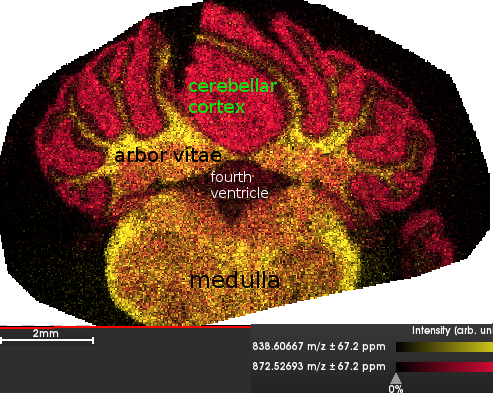
\includegraphics[width=1\textwidth]{raw/hirn/Hirn872-838_ann}
    \caption{Annotierte MALDI-Imaging-Aufnahme eines Coronal-Schnittes eines Mäusehirns.}
    \label{fig:hirn-ann}
\end{figure}

	\newpage
\section{Schlussfolgerung}
	% Rückgriff auf Hypothese und drittes Nennen dieser
	% Quellen zitieren, Websiten mit Zugriffsdatum
	% Verweise auf das Laborbuch (sind erlaubt)
	% Tabelle + Bilder mit Beschriftung

  Zusammenfassend lässt sich sagen, dass 

		% --- Anhang einbinden
	\newpage
\appendix
\newpage
\section{Anhang}\label{sec:anhang}

%\subsection{Unsicherheiten}\label{sec:unsicherheiten}

Alle Unsicherheiten werden nach dem GUM bestimmt und berechnet.
Die Gleichungen dazu finden sich in \ref{fig:GUM_combine} und \ref{fig:GUM_formula}.
Hierfür wurde die Python Bibliothek \enquote{uncertainties} verwendet, welche den Richtlinien des GUM folgt.
Für die Unsicherheiten der Parameter in Annäherungskurven wurden die $y$-Unsicherheiten der anzunähernden Werte beachtet und die Methode der kleinsten Quadrate angewandt.
Dafür steht in der Bibliothek die Methode \enquote{scipy.optimize.curve\_fit()} zur Verfügung.

Für Messungen mit digitalen Anzeigen wird eine rechteckige Verteilung mit $\sigma_X = \frac{\Delta X}{2\sqrt{3}}$ aufgrund der begrenzten Ziffernzahl und für analoges Ablesen wird eine Dreiecksverteilung mit $\sigma_X = \frac{\Delta X}{2\sqrt{6}}$ angenommen.
Die jeweiligen $\Delta X$ sind im entsprechenden Abschnitt zu finden.

\begin{figure}[ht]
	\begin{equation*}
	x = \sum_{i=1}^{N} x_i
	;\quad
	\sigma_x = \sqrt{\sum_{i = 1}^{N} \sigma_{x_i}^2}
	\end{equation*}
	\caption{Formel für kombinierte Unsicherheiten des selben Typs nach GUM.}
	\label{fig:GUM_combine}
\end{figure}

\begin{figure}[ht]
	\begin{align*}
	f = f(x_1, \dots , x_N)
	;\quad
	\sigma_f = \sqrt{\sum_{i = 1}^{N}\left(\pdv{f}{x_i} \sigma_{x_i}\right) ^2}
	\end{align*}
	\caption{Formel für sich fortpflanzende Unsicherheiten erster Ordnung nach GUM.}
	\label{fig:GUM_formula}
\end{figure}

\begin{table}[H]
	\centering
	\caption{Ergebnisse aus den Fits ausgewählter Peaks in den Massenspektren. MVM meint Matrix, Verdünnungsstufe ($\log_{10}(c \cdot \si{\liter \per \mole})$) und Modus des Flugzeitspektrometers (HR/S). SRV ist das Signal-Rausch-Verhältnis.}
	\resizebox{\textwidth}{!}{%
	\begin{tabular}{c | c | c | c | c}
MVM & Position ($m/z$) & Halbwertsbreite & Massenauflösung $R$ & SRV \\ \hline
DHB-7S	& \SI{ 734.57044 \pm 0.00023 }{} & \SI{ 0.0563 \pm 0.0006 }{} & \SI{ 1.304 \pm 0.013e+04 }{} & \SI{ 101 \pm 27 }{}\\
	& \SI{ 760.58588 \pm 0.00021 }{} & \SI{ 0.0596 \pm 0.0005 }{} & \SI{ 1.277 \pm 0.011e+04 }{} & \SI{ 90 \pm 19 }{}\\
DHB-7S	& \SI{ 734.57001 \pm 0.00020 }{} & \SI{ 0.0560 \pm 0.0005 }{} & \SI{ 1.312 \pm 0.012e+04 }{} & \SI{ 85 \pm 17 }{}\\
	& \SI{ 760.58550 \pm 0.00026 }{} & \SI{ 0.0612 \pm 0.0007 }{} & \SI{ 1.243 \pm 0.013e+04 }{} & \SI{ 51 \pm 7 }{}\\
DHB-6S	& \SI{ 734.5691 \pm 0.0007 }{} & \SI{ 0.0602 \pm 0.0017 }{} & \SI{ 1.219 \pm 0.035e+04 }{} & \SI{ 17.2 \pm 2.1 }{}\\
	& \SI{ 760.5853 \pm 0.0006 }{} & \SI{ 0.0626 \pm 0.0016 }{} & \SI{ 1.214 \pm 0.032e+04 }{} & \SI{ 21.3 \pm 3.0 }{}\\
DHB-5S	& \SI{ 734.57021 \pm 0.00023 }{} & \SI{ 0.0566 \pm 0.0006 }{} & \SI{ 1.298 \pm 0.013e+04 }{} & \SI{ 81 \pm 17 }{}\\
	& \SI{ 760.58573 \pm 0.00025 }{} & \SI{ 0.0580 \pm 0.0006 }{} & \SI{ 1.312 \pm 0.015e+04 }{} & \SI{ 108 \pm 33 }{}\\
CHCA-5S	& \SI{ 734.57025 \pm 0.00024 }{} & \SI{ 0.0553 \pm 0.0006 }{} & \SI{ 1.329 \pm 0.015e+04 }{} & \SI{ 65 \pm 12 }{}\\
	& \SI{ 760.58590 \pm 0.00022 }{} & \SI{ 0.0601 \pm 0.0006 }{} & \SI{ 1.266 \pm 0.012e+04 }{} & \SI{ 74 \pm 13 }{}\\
DHB-4HR	& \SI{ 734.56227 \pm 0.00018 }{} & \SI{ 0.0217 \pm 0.0004 }{} & \SI{ 3.39 \pm 0.07e+04 }{} & \SI{ 1.0 \pm 0.5e+02 }{}\\
	& \SI{ 760.5789 \pm 0.0004 }{} & \SI{ 0.0212 \pm 0.0009 }{} & \SI{ 3.58 \pm 0.16e+04 }{} & \SI{ 1.6 \pm 2.4e+02 }{}\\
DHBA-4S	& \SI{ 734.56961 \pm 0.00022 }{} & \SI{ 0.0485 \pm 0.0005 }{} & \SI{ 1.516 \pm 0.017e+04 }{} & \SI{ 1.4 \pm 0.5e+02 }{}\\
	& \SI{ 760.58515 \pm 0.00022 }{} & \SI{ 0.0504 \pm 0.0006 }{} & \SI{ 1.509 \pm 0.017e+04 }{} & \SI{ 1.4 \pm 0.5e+02 }{}\\
	& \SI{ 734.56547 \pm 0.00008 }{} & \SI{ 0.01889 \pm 0.00021 }{} & \SI{ 3.89 \pm 0.04e+04 }{} & \SI{ 1.9 \pm 0.6e+02 }{}\\
	& \SI{ 760.58107 \pm 0.00011 }{} & \SI{ 0.01993 \pm 0.00026 }{} & \SI{ 3.82 \pm 0.05e+04 }{} & \SI{ 3.1 \pm 2.0e+02 }{}\\
DHB-4H	& \SI{ 734.56532 \pm 0.00009 }{} & \SI{ 0.01984 \pm 0.00023 }{} & \SI{ 3.70 \pm 0.04e+04 }{} & \SI{ 1.8 \pm 0.6e+02 }{}\\
	& \SI{ 760.58040 \pm 0.00030 }{} & \SI{ 0.0211 \pm 0.0008 }{} & \SI{ 3.61 \pm 0.13e+04 }{} & \SI{ 1.6 \pm 2.9e+02 }{}\\
DHB-4S	& \SI{ 734.56939 \pm 0.00020 }{} & \SI{ 0.0508 \pm 0.0005 }{} & \SI{ 1.445 \pm 0.014e+04 }{} & \SI{ 1.5 \pm 0.5e+02 }{}\\
	& \SI{ 760.58470 \pm 0.00021 }{} & \SI{ 0.0515 \pm 0.0005 }{} & \SI{ 1.477 \pm 0.015e+04 }{} & \SI{ 1.4 \pm 0.5e+02 }{}\\
DHB-4S	& \SI{ 734.56954 \pm 0.00023 }{} & \SI{ 0.0513 \pm 0.0006 }{} & \SI{ 1.433 \pm 0.016e+04 }{} & \SI{ 1.3 \pm 0.4e+02 }{}\\
	& \SI{ 760.58489 \pm 0.00020 }{} & \SI{ 0.0542 \pm 0.0005 }{} & \SI{ 1.404 \pm 0.013e+04 }{} & \SI{ 1.5 \pm 0.5e+02 }{}\\
CHCA-4HR	& \SI{ 734.56593 \pm 0.00027 }{} & \SI{ 0.0183 \pm 0.0007 }{} & \SI{ 4.02 \pm 0.15e+04 }{} & \SI{ 1.2 \pm 1.1e+02 }{}\\
	& \SI{ 760.58217 \pm 0.00014 }{} & \SI{ 0.01832 \pm 0.00034 }{} & \SI{ 4.15 \pm 0.08e+04 }{} & \SI{ 2.3 \pm 2.0e+02 }{}\\
CHC-4S	& \SI{ 734.56831 \pm 0.00018 }{} & \SI{ 0.0576 \pm 0.0005 }{} & \SI{ 1.276 \pm 0.010e+04 }{} & \SI{ 113 \pm 26 }{}\\
	& \SI{ 760.58334 \pm 0.00018 }{} & \SI{ 0.0605 \pm 0.0005 }{} & \SI{ 1.257 \pm 0.010e+04 }{} & \SI{ 1.5 \pm 0.4e+02 }{}\\
CHCA-4HR	& \SI{ 734.56643 \pm 0.00018 }{} & \SI{ 0.0188 \pm 0.0004 }{} & \SI{ 3.91 \pm 0.09e+04 }{} & \SI{ 83 \pm 30 }{}\\
	& \SI{ 760.58104 \pm 0.00021 }{} & \SI{ 0.0203 \pm 0.0005 }{} & \SI{ 3.75 \pm 0.09e+04 }{} & \SI{ 2.6 \pm 3.0e+02 }{}\\
	& \SI{ 734.5637 \pm 0.0004 }{} & \SI{ 0.0183 \pm 0.0009 }{} & \SI{ 4.02 \pm 0.20e+04 }{} & \SI{ 1.0 \pm 0.9e+02 }{}\\
	& \SI{ 760.58013 \pm 0.00025 }{} & \SI{ 0.0209 \pm 0.0006 }{} & \SI{ 3.64 \pm 0.11e+04 }{} & \SI{ 2.5 \pm 3.1e+02 }{}\\
CHCA-4S	& \SI{ 734.56806 \pm 0.00024 }{} & \SI{ 0.0579 \pm 0.0006 }{} & \SI{ 1.268 \pm 0.013e+04 }{} & \SI{ 108 \pm 31 }{}\\
	& \SI{ 760.58363 \pm 0.00021 }{} & \SI{ 0.0585 \pm 0.0005 }{} & \SI{ 1.301 \pm 0.012e+04 }{} & \SI{ 121 \pm 35 }{}\\
	\end{tabular}
	}
	\label{tab:massiv}
\end{table}

		
	\printbibliography


\end{document}
